\chapter{Experiments}
\label{chap:experiments}

As mentioned in this thesis' introduction, adaptive beamformers have often been criticized as not reliable enough in their raw form for most active system applications such as medical ultrasound imaging.
Some of the early concerns such beamformers faced included their notable sensitivity to:
\begin{enumerate}
    \item Signal cancellation in the presence of coherent signals (\cite{van_trees})
    \item Visible artifacts in the presence of motion in the imaged medium (\cite{Asen_shift_invariance})
    \item High beam density requirements due to narrow receive beams
    \item High computational complexity prohibiting real-time ultrasound imaging
    \item High configuration complexity
\end{enumerate}
\noindent
Different approaches have been proposed to solve or limit the effect of one issue or another, some of which are presented in this thesis (Sections \ref{sec:diagonal_loading} - \ref{sec:multibeam}).
Multiple studies have compared different versions of the MV beamformers with the DAS one (\cite{Synnevag_Benefits, Synnevag_adaptive, Asen_shift_invariance}), both in idle scenarios and in scenarios exposed to motion. One objective of this thesis is to build experiments that create similar comparisons and hopefully confirm the conclusions of these publications. This aims to provide confidence in the experiments and analysis with new content.

The multibeam Iterative Adaptive Approach (IAA-MB) has been presented in ultrasound image processing by \cite{Jensen_IAA} as an alternative beamformer to MV. Although very promising, it has only been studied in medical ultrasound imaging on scenarios with stationary imaged media. The effects of motion on the IAA-MB approach is an aspect that this thesis hopes to explore and uncover.

In the domain of medical ultrasound imaging, motion in an imaged medium is often, implicitly or explicitly, defined as position shift of scatterer points from one image, or frame, to another. However, the acquisition of a single frame is not instantaneous, which means that motion within a frame is a real concept and a potential source of issues for different beamformers. This thesis aims to provide a thorough analysis of the effects of motion within frames and the resulting limitations on each beamformer.

The combined analysis of all scenarios experimented with in this thesis is expected to provide a reliable and thorough understanding of the fundamental issues and artifacts induced from motion in ultrasound imaging, along with realistic limitations, and enhancement possibilities, of each beamformer presented in this thesis.

\section{The effect of motion between frames}
\label{sec:frames_motion}
This section aims to compare how well each beamformer copes with motion between frames. \cite{Asen_shift_invariance} already revealed results comparing the MV beamformer with DAS. The goal of this section is to build on this study, hopefully confirm its findings, and provide a similar analysis for the different versions of the IAA approach presented in this thesis.

The for-mentioned study showed that the MV algorithm requires a much higher beam density than DAS in order to ensure no visible artifact. Due to the MV beams being very narrow at the radial focus, the reflections from scatterer points located in between two beams focus points can be heavily attenuated compared to scatterer points located at a beam focus point. This signal attenuation effect is known as \textit{scalloping loss} (\cite{Asen_shift_invariance}). In the case of a moving scatterer point, this scalloping loss effect will result in the point's apparent intensity varying with its position. When combining beamformed images into videos, as done for example in real-time imaging,  scatterer points in motion may appear blinking. Figure \ref{fig:bf_im} illustrates the effect of scalloping loss with the DAS beamformer. A single scatterer point is simulated in a speckle noise background. The white lines indicate transmit beams trajectories. The scatterer point starts on the center beam trajectory and is shifted half the distance between two beams per frame, such that it ends exactly on the neighboring beam trajectory in the third frame. In this example, the scatterer point is visible in frames 1 and 3, but completely disappears in the speckle background in frame 2.

\begin{figure}[ht]
    \centering
    \begin{subfigure}[t]{0.48\linewidth}
        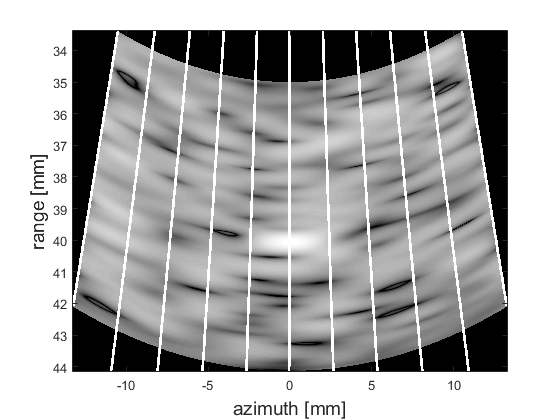
\includegraphics[width=\linewidth]{./images/others/scallop_loss1.png}
        \caption{Position of $s_1 = (0, 40)~$mm.}
        \label{fig:bf_im1}
    \end{subfigure}
    \quad
    \begin{subfigure}[t]{0.48\linewidth}
        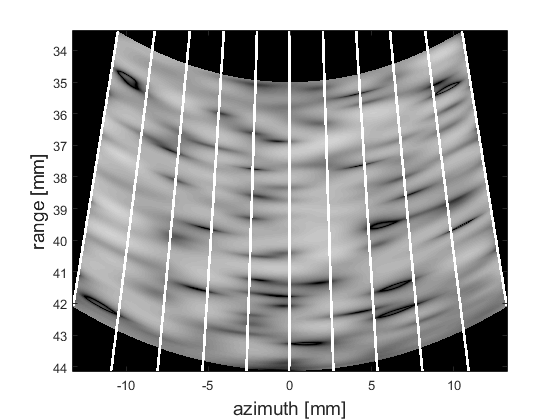
\includegraphics[width=\linewidth]{./images/others/scallop_loss2.png}
        \caption{Position of $s_1 = (1.2, 39.98)~$mm.}
        \label{fig:bf_im2}
    \end{subfigure}
    \quad
    \begin{subfigure}[t]{0.48\linewidth}
        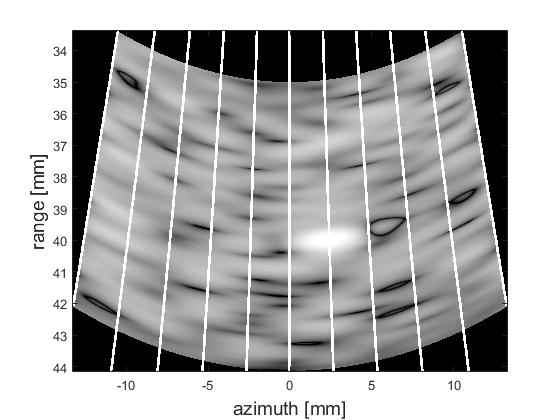
\includegraphics[width=\linewidth]{./images/others/scallop_loss3.png}
        \caption{Position of $s_1 = (2.4, 39.93)~$mm.}
        \label{fig:bf_im3}
    \end{subfigure}
    \caption[DAS beamformed images of a scatterer point $s_1$ moving in speckle.]{DAS beamformed images of a scatterer point $s_1$ moving in speckle. The scatterer point is shifted, along the beamformer's focus radius, half the distance between beams per frame. The position $(x, y)$ of $s_1$ is $(0, 40)~$mm in (a), $(1.2, 39.98)~$mm in (b) and $(2.4, 39.93)~$mm in (c), where $x$ is the offset of $s_1$ relative to the center of the array along the azimuth dimension and $y$ is the offset along the range dimension. The white lines are added on top of the beamformed image and represent the transmit beams trajectories.}
	\label{fig:bf_im}
\end{figure}

Scalloping loss, for any scatterer point in the medium, can be caused by a lack of energy transmitted towards the point's position or by signal suppression from the array towards that position.
Two of the most straightforward approaches to reducing scalloping loss are by either increasing the density of transmit beams or their width. However both methods have obvious drawbacks. The choice of beam width is a trade-off between sensitivity to scalloping loss and image resolution, whereas the choice of their density is a trade-off between sensitivity to scalloping loss and image acquisition time.

A beamformed image is considered in this thesis to be formed by sequentially transmitting and recording focused beams. Its acquisition time $t_{im}$ can be expressed in seconds as:
\begin{equation}
    t_{im} = 2 \cdot r_{max} \cdot b_{tr} / c,
\label{eq:acquisition_time}
\end{equation}
\noindent
where $b_{tr}$ is the number of transmit beams, $r_{max}$ is the maximum range in meters for which the probe is recording data and $c$, in m/s, is the speed of ultrasound propagation in the medium. The factor 2 represents the fact that active systems are used, which means that the signals need to travel to $r_{max}$ and back to the probe in order to be recorded. With $r_{max} = 0.15~$m and $c = 1500~$m/s, $t_{im} = 2 \cdot 0.15 \cdot b_{tr} / 1500 =  2 \cdot 10^{-4} \cdot b_{tr}~$seconds. A single beam transmission and acquisition is then considered to take $0.2~$ms.

Instead of acquisition time, it is often slightly more intuitive to talk about frame rate, in number of images per second, especially in the domain of real-time imaging. The beamformers' frame rate $f_{im}$ are calculated through this thesis as:
\begin{equation}
    f_{im} = 1 / t_{im} = 1 / (2 \cdot 10^{-4} \cdot b_{tr}) = 5 \cdot 10^3 / b_{tr}.
\label{eq:frame_rate}
\end{equation}
\noindent
A beamformer's frame rate is dependent on the number of transmit beams $b_{tr}$, but not dependent on the number of receive beams $b_{re}$. For beamformers using single-line acquisition (SLA), those number are equal. However, as explained in Section \ref{sec:prb}, multi-line acquisition (MLA) is an approach that can create multiple receive beams per transmit beam and output beamformed images with $b_{re} > b_{tr}$.
Given an image resolution threshold, MLA approaches can often be used to reduce the required transmit beam density compared to that of the SLA approach, thus increasing a beamformer's maximum frame rate.

Since data processing and acquisition can often be done simultaneously and computation capabilities are constantly increasing, we focus in this thesis on analyzing delays due to data acquisition and assume data processing can be made such that it does not result in additional delays.
In order to avoid potential artifacts, the whole imaged medium is considered to be idle within a single frame. The effects of motion within frames are studied in Section \ref{sec:beams_motion}.

In order to give a meaningful interpretation of the effects of scalloping loss, and qualitatively compare these results with previous studies, the scalloping visibility threshold is taken from \cite{Asen_shift_invariance}: \newline
\textit{In an ultrasound image with 50dB dynamic range mapped to 256 gray levels, a 1dB loss corresponds to 5 gray levels. This is approximately equal to the visibility threshold [Weber fraction of 2\%] for grayscale images. A loss larger than 1dB could therefore end up being visible to the observer.}

Since focused beams are by definition the narrowest at their radial focus, it is the range at which the scalloping loss of scatterer points is expected to be the most severe. This assumption has to be verified before comparing beamformers performance at radial focus.
To simulate the highest possible scalloping loss, the scatterer point motion follows the aperture's focus radius and is therefore physically a circular motion. Multiple frames are recorded with the point at different angles from the aperture's center. The maximum scatterer point gain is expected to be recorded when its angle matches one of the array's beams. Its minimum gain is expected to be recorded when its angle is exactly in between two beams angle. The scatterer point maximum scalloping loss is then calculated by subtracting its estimated minimum gain to its estimated maximum gain.


\section{The effect of motion within frames}
\label{sec:beams_motion}
In Section \ref{sec:frames_motion}, the back-scattered image was assumed to be still within each frame. This section is analyzing the effects of motion within a single frame. This domain has been very little studied so far in medical ultrasound imaging, which makes it harder to predict the outcome of such experiments. However this might hint that motion within frames has not revealed any known major issue for conventional beamformers and might only induce negligible errors in the beamformers model. The purpose of this section is to analyze the effects of such motion and give sensible information about how robust the different beamformers are in realistic scenarios.

The domain of photography, although fundamentally different in its signal acquisition process from ultrasound beamforming, is dramatically affected by motion within frames. Almost anybody who has ever handled a camera has experienced motion in the imaged scenery leading to blur in the image. This experience, perhaps misleadingly, directs us to expect such motion in the ultrasound imaging domain to result in distortions of the scatterer points shape and amplitude.

In order to give more insightful predictions, it is worth analyzing the photography analogy a bit deeper. First of all, cameras capture frames by recording light waves simultaneously for the whole spatial spectrum. The reason blur or artifacts can appear is that the frame's capture is not instantaneous. The camera's \textit{exposure time} is what defines how long a frame is recorded for. A long exposure time allows us to record a lot of light and get brighter pictures. A short exposure time limits the effects of motion blur, but also results in darker pictures. This process can be seen as continuously taking instantaneous frame for a given period and produce the final picture by averaging those frames. If an object moves during that time, it can appear blurry since not at the same spatial location for all frames. Motion in any direction would then result in the object appearing bigger than if idle. 

In ultrasound imaging, the probes are typically sending short pulses which are reflected by scatterers in the imaged medium. In such scenarios, with only a few samples per range pixel, motion in the medium within a single beam is way beyond human perception for velocities $v << c$, the speed of ultrasound propagation, and can be ignored. However, blur and artifacts can occur due to the sequential nature of image acquisition, i.e. the formation and recording of directional beams. Frames are produced by transmitting and recording directional beams along the imaged spatial spectrum. In this thesis, the beams are transmitted sequentially from negative to positive degrees/azimuth. Each beam needs to propagate until the desired maximum image range and back to the array before another beam can be transmitted. The image acquisition time is defined by Equation (\ref{eq:acquisition_time}).

In the photography analogy, it would be similar to taking a panoramic picture, where picture frames are extended by other ones in order to form a picture with extended spatial range. Assuming this time that each picture is instantaneous, no blur or artifact can occur within a single picture. For simplicity, it is first considered that all pictures are forming a perfectly aligned panoramic picture, with no overlap in their imaged sector. Multiple scenarios of a single object moving in a stationary background are then proposed in Table \ref{table:panoramic_perfect}, where the object motion $\boldsymbol{m_o}$ is expressed relative to the panoramic picture acquisition direction $\boldsymbol{m_p}$.

With these initial intuitions in mind, the photography analogy can be extended to the scenario for which the different pictures overlap in their imaged sector. The same scenes as Table \ref{table:panoramic_perfect} are analyzed with pictures overlap in Table \ref{table:panoramic_imperfect}.

\begin{table}[!ht]
\centering
\begin{tabular}{| c | c |}
  \hline
  \textbf{Scenario}  &   \textbf{Expected result} \\
  \hline
  Object appears only in one frame    &   No artifact or blur \\
  \hline
  $\boldsymbol{m_o}$ in same direction as $\boldsymbol{m_p}$  &  The object can appear dilated, or, in \\
    &  extreme cases, a duplicate can appear \\
  \hline
  $\boldsymbol{m_o}$ opposite to $\boldsymbol{m_p}$    &  The object can appear eroded   \\
    &   or, in extreme cases, disappear \\
  \hline
  $\boldsymbol{m_o}$ perpendicular to $\boldsymbol{m_p}$    &   The object can appear distorted \\
  \hline
 \end{tabular}
\caption{Photography analogy of an object moving in between frames of a panoramic picture. Expected artifacts with perfect image segmentation.}
\label{table:panoramic_perfect}
\end{table}


\begin{table}[!ht]
\centering
\begin{tabular}{| c | c |}
  \hline
  \textbf{Scenario}  &   \textbf{Expected result} \\
  \hline
  Object appears only in one frame    &   No artifact or blur \\
  \hline
    &  The object can appear blurry, \\
  $\boldsymbol{m_o}$ in same direction as $\boldsymbol{m_p}$  &   dilated or, in extreme cases,  \\
    &   a duplicate can appear   \\
  \hline
  $\boldsymbol{m_o}$ opposite to $\boldsymbol{m_p}$    &  The object can appear \\
    &   blurry or eroded  \\
  \hline
  $\boldsymbol{m_o}$ perpendicular to $\boldsymbol{m_p}$    &   The object can appear \\
    &   blurry or distorted \\
  \hline
 \end{tabular}
\caption{Photography analogy of an object moving in between frames of a panoramic picture. Expected artifacts with imperfect image segmentation.}
\label{table:panoramic_imperfect}
\end{table}

The first part of this section aims to give a first exposure to the effects and possible issues of motion within frames. The assumptions of Tables \ref{table:panoramic_imperfect} and \ref{table:panoramic_perfect} made from the photography analogy are then compared to the results in medical ultrasound imaging. Different motion patterns and velocities are studied with a single scatterer point at the array's focus range, in a noiseless background. Then, the same analysis is done with the presence of speckle noise, in order to confirm or disprove the conclusions made from the first analysis.

Blood flow velocities in arteries are typically on average around 0.12 m/s, with peaks around 0.6 m/s (\cite{Blood_flow}). With this in mind, this section's analysis focuses on the 0 to 0.6 m/s velocity range.
The second part of this section analyses the effect of motion with multiple scatterer points in an attempt to discover any potential additional effect in scenarios with coherent signals. The experiments run are very similar to those of the first part of this section, although with the presence of signal coherence induced by two closely-separated scatterer points in the imaged medium.
